\documentclass[12pt,a4paper]{article}
\usepackage[margin=2cm]{geometry}
\usepackage{xeCJK}
\usepackage{fontspec}
\setCJKmainfont{Noto Serif CJK TC}[Script=CJK]
\usepackage{amsmath,amssymb}
\usepackage{graphicx}
\usepackage{fancyhdr}
\setlength{\headheight}{14.5pt}
\addtolength{\topmargin}{-2.5pt}
\usepackage{hyperref}
\usepackage{listings}
\usepackage{enumitem}
\usepackage{titlesec}
\usepackage{caption}
\usepackage{indentfirst}
\usepackage{booktabs}
\usepackage{longtable}
\usepackage{multirow}
\usepackage{array}
\usepackage{tabularx}
\usepackage{float}
\usepackage{algorithm}
\usepackage{algpseudocode}
\usepackage{minted}
\setlength{\parindent}{2em}
\pagestyle{fancy}
\fancyhf{}
\cfoot{\thepage}
\linespread{1.3}
\setminted{
    linenos,                % 行號
    frame=lines,            % 上下框線
    framesep=5pt,           % 程式碼與邊框距離
    numbersep=8pt,          % 行號與程式碼距離
    fontsize=\scriptsize,   % 字體大小
    breaklines,             % 自動換行
    tabsize=4,              % tab 寬度
    rulecolor=\color{black},% 框線顏色
    xleftmargin=1.5em       % 左側縮排
}

\title{Machine Learning Homework 1}
\author{B12508026戴偉璿}
\date{\today}

\begin{document}

\maketitle

\lhead{Machine Learning Homework 1}
\rhead{B12508026戴偉璿}
\newpage
\tableofcontents
\newpage

\section{Problem 1}

\subsection{Bayesian Decision Model}
\subsubsection{Model Description}
In this homework, I implement a Bayesian Decision Model to classify data points based on their features. The model assumes that the data points are generated from a mixture of Gaussian distributions, each corresponding to a different class.

A multivariate Gaussian distribution is defined as follows:
\begin{equation}
p(\mathbf{x}|\mu, \Sigma) = \frac{1}{(2\pi)^{d/2} |\Sigma|^{1/2}} \exp\left(-\frac{1}{2}(\mathbf{x}-\mu)^T \Sigma^{-1} (\mathbf{x}-\mu)\right)
\end{equation}
where $\mu$ is the mean vector, $\Sigma$ is the covariance matrix, and $d$ is the dimensionality of the data.

\subsubsection{Parameter Estimation}
To estimate the parameters of the Gaussian distributions for each class, I need the prior probabilities $P(C_i)$, the mean vectors $\mu_i$, and the covariance matrices $\Sigma_i$ for each class $C_i$. 

The prior probabilities are estimated as follow, $N_i$ is the number of samples in class $C_i$ and $N$ is the total number of samples.
\begin{equation}
P(C_i) = \frac{N_i}{N}
\end{equation}

The mean vector for each class is estimated as:
\begin{equation}
\mu_i = \frac{1}{N_i} \sum_{x \in C_i} x
\end{equation}

The covariance matrix for each class is estimated as:
\begin{equation}
\Sigma_i = \frac{1}{N_i} \sum_{x \in C_i} (x - \mu_i)(x - \mu_i)^T
\end{equation}

\subsubsection{Feature Selection}
In this homework, I implement a forward feature selection algorithm to select the best subset of features that maximizes the model's performance. The algorithm starts with an empty set of features and iteratively adds the feature that results in the highest increase in performance, measured by the Area Under the Curve (AUC) of the Receiver Operating Characteristic (ROC) curve.

The algorithm for the forward feature selection algorithm is as follows:
\begin{algorithm}[H]
\caption{Forward Feature Selection (FFS)}
\label{alg:ffs}
\begin{algorithmic}[1]
\Require Dataset $D = \{(X_{\text{train}}, X_{\text{test}}, y_{\text{train}}, y_{\text{test}})\}$, feature dimension $d$
\Ensure Best feature mask $\text{best\_mask}$, best AUC $\text{best\_auc}$, best posterior $\text{best\_prior}$

\State Initialize $\text{best\_mask} \gets [0, 0, \dots, 0]$ 
\State Initialize $\text{best\_auc} \gets 0.0$

\Repeat
    \State $\text{local\_best\_auc} \gets -1$
    \State $\text{local\_best\_mask} \gets \text{best\_mask}$
    \For{$i = 1$ to $d$}
        \If{$\text{best\_mask}[i] = 1$}
            \State \textbf{continue}
        \EndIf
        \State $\text{local\_mask} \gets \text{best\_mask}$; $\text{local\_mask}[i] \gets 1$
        \State Train model with $\text{local\_mask}$ to get AUC $\text{auc}_i$ and posterior $\text{prior}_i$
        \If{$\text{auc}_i > \text{local\_best\_auc}$}
            \State $\text{local\_best\_auc} \gets \text{auc}_i$
            \State $\text{local\_best\_mask} \gets \text{local\_mask}$
            \State $\text{local\_best\_prior} \gets \text{prior}_i$
        \EndIf
    \EndFor
    \If{$\text{local\_best\_auc} \le \text{best\_auc}$}
        \State \textbf{break}
    \Else
        \State $\text{best\_auc} \gets \text{local\_best\_auc}$
        \State $\text{best\_mask} \gets \text{local\_best\_mask}$
        \State $\text{best\_prior} \gets \text{local\_best\_prior}$
    \EndIf
\Until{no improvement in AUC}

\State \Return $\text{best\_auc}, \text{best\_mask}, \text{best\_prior}$
\end{algorithmic}
\end{algorithm}

Following is the feature selected in each fold:
\begin{minted}{bash}
Fold 1: ['FaceWM', 'FaceWmax', 'Na-Chin', 'LFaceH', 'MouthW', 'LVermilionH', 'LVermilionC', 'NoseVol', 'NoseW', 'NasoFacialA']
Fold 2: ['FaceWM', 'FaceWL', 'FaceWmax', 'Na-Chin', 'LFaceH', 'MouthW', 'LVermilionH', 'LVermilionC', 'NoseSurfA', 'NoseW', 'NasoFacialA']
Fold 3: ['FaceWM', 'FaceWmax', 'Na-Chin', 'LFaceH', 'MouthW', 'LVermilionH', 'LVermilionC', 'NoseVol', 'NoseW', 'NasoFacialA']
Fold 4: ['FaceWM', 'FaceWL', 'FaceWmax', 'Na-Chin', 'Subn-Chin', 'LFaceH', 'LipH', 'UVermilionH', 'LVermilionH', 'UVermilionC', 'LVermilionC', 'NoseVol', 'NoseW', 'NasoFacialA']
Fold 5: ['FaceWM', 'FaceWmax', 'Na-Chin', 'Subn-Chin', 'LFaceH', 'LipH', 'UVermilionH', 'LVermilionH', 'UVermilionC', 'LVermilionC', 'NoseVol', 'NoseW', 'NasoFacialA']
Fold 6: ['FaceWM', 'FaceWmax', 'Subn-Chin', 'MouthW', 'LVermilionH', 'NoseVol', 'NoseW', 'NasoFacialA']
Fold 7: ['FaceWM', 'FaceWL', 'FaceWmax', 'Na-Chin', 'Subn-Chin', 'LFaceH', 'LipH', 'UVermilionH', 'LVermilionH', 'UVermilionC', 'LVermilionC', 'NoseVol', 'NoseW', 'NasoFacialA']
Fold 8: ['FaceWM', 'FaceWmax', 'MFaceH', 'LFaceH', 'MouthW', 'LVermilionH', 'LVermilionC', 'NoseVol', 'NoseW', 'NasoFacialA']
Fold 9: ['FaceWM', 'FaceWmax', 'Na-Chin', 'LFaceH', 'MouthW', 'LVermilionH', 'LVermilionC', 'NoseVol', 'NoseW', 'NasoFacialA']
Fold 10: ['FaceWM', 'FaceWmax', 'Na-Chin', 'LFaceH', 'MouthW', 'LVermilionH', 'LVermilionC', 'NoseVol', 'NoseW', 'NasoFacialA']
Fold 11: ['FaceWM', 'FaceWmax', 'Subn-Chin', '   LipD   ', 'MFaceH', 'LFaceH', 'MouthW', 'LipH', 'UVermilionH', 'LVermilionH', 'UVermilionC', 'LVermilionC', 'NoseVol', 'NasoFacialA']
Fold 12: ['FaceWM', 'FaceWmax', 'Na-Chin', 'LFaceH', 'MouthW', 'LVermilionH', 'LVermilionC', 'NoseVol', 'NoseW', 'NasoFacialA']
Fold 13: ['FaceWM', 'FaceWmax', 'Na-Chin', 'LFaceH', 'MouthW', 'LVermilionH', 'LVermilionC', 'NoseVol', 'NoseW', 'NasoFacialA']
Fold 14: ['FaceWM', 'FaceWmax', 'Na-Chin', 'LFaceH', 'MouthW', 'LVermilionH', 'LVermilionC', 'NoseVol', 'NoseW', 'NasoFacialA']
Fold 15: ['FaceWM', 'FaceWmax', 'Na-Chin', 'LFaceH', 'MouthW', 'LVermilionH', 'LVermilionC', 'NoseVol', 'NoseW', 'NasoFacialA']
Fold 16: ['FaceWM', 'FaceWL', 'FaceWmax', 'MFaceH', 'LFaceH', 'MouthW', 'LVermilionH', 'LVermilionC', 'NoseVol', 'NoseW', 'NasoFacialA']
Fold 17: ['FaceWM', 'FaceWmax', 'Na-Chin', 'LFaceH', 'MouthW', 'LVermilionH', 'LVermilionC', 'NoseVol', 'NoseW', 'NasoFacialA']
Fold 18: ['FaceWM', 'FaceWmax', 'Na-Chin', 'LFaceH', 'MouthW', 'LVermilionH', 'LVermilionC', 'NoseVol', 'NoseW', 'NasoFacialA']
Fold 19: ['FaceWM', 'FaceWmax', 'Na-Chin', 'LFaceH', 'MouthW', 'LVermilionH', 'LVermilionC', 'NoseVol', 'NoseW', 'NasoFacialA']
Fold 20: ['FaceWM', 'FaceWmax', 'Na-Chin', 'LFaceH', 'MouthW', 'LVermilionH', 'UVermilionC', 'LVermilionC', 'NoseVol', 'NoseW', 'NasoFacialA']
Fold 21: ['FaceWM', 'FaceWmax', 'Na-Chin', 'LFaceH', 'MouthW', 'LVermilionH', 'LVermilionC', 'NoseVol', 'NoseW', 'NasoFacialA']
Fold 22: ['FaceWL', 'FaceWmax', 'Na-Chin', 'LFaceH', 'LVermilionH', 'LVermilionC', 'NoseVol', 'NoseW', 'NasoFacialA']
Fold 23: ['FaceWM', 'FaceWmax', 'Na-Chin', 'LFaceH', 'MouthW', 'LVermilionH', 'LVermilionC', 'NoseVol', 'NoseW', 'NasoFacialA']
Fold 24: ['FaceWL', 'FaceWmax', 'Na-Chin', 'LFaceH', 'LVermilionH', 'NoseVol', 'NoseW', 'NasoFacialA']
Fold 25: ['FaceWM', 'FaceWmax', 'Na-Chin', 'LFaceH', 'MouthW', 'LVermilionH', 'LVermilionC', 'NoseVol', 'NoseW', 'NasoFacialA']
Fold 26: ['FaceWM', 'FaceWL', 'FaceWmax', 'Na-Chin', 'Subn-Chin', 'LFaceH', 'LipH', 'UVermilionH', 'LVermilionH', 'UVermilionC', 'LVermilionC', 'NoseVol', 'NoseW', 'NasoFacialA']
Fold 27: ['FaceWM', 'FaceWmax', 'Na-Chin', 'LFaceH', 'MouthW', 'LVermilionH', 'LVermilionC', 'NoseVol', 'NoseW', 'NasoFacialA']
Fold 28: ['FaceWM', 'FaceWL', 'FaceWmax', 'MFaceH', 'LFaceH', 'MouthW', 'LVermilionH', 'LVermilionC', 'NoseVol', 'NoseW', 'NasoFacialA']
Fold 29: ['FaceWM', 'FaceWL', 'FaceWmax', 'Na-Chin', 'Subn-Chin', 'LFaceH', 'LipH', 'UVermilionH', 'LVermilionH', 'UVermilionC', 'LVermilionC', 'NoseVol', 'NoseW', 'NasoFacialA']
Fold 30: ['FaceWM', 'FaceWL', 'FaceWmax', 'Na-Chin', 'Subn-Chin', 'LFaceH', 'LipH', 'UVermilionH', 'LVermilionH', 'UVermilionC', 'LVermilionC', 'NoseVol', 'NoseW', 'NasoFacialA']
Fold 31: ['FaceWM', 'FaceWL', 'FaceWmax', 'Na-Chin', 'Subn-Chin', 'MFaceH', 'LVermilionH', 'LVermilionC', 'NoseVol', 'NoseW', 'NasoFacialA']
Fold 32: ['FaceWM', 'FaceWL', 'FaceWmax', 'Na-Chin', 'Subn-Chin', 'LFaceH', 'LipH', 'UVermilionH', 'LVermilionH', 'UVermilionC', 'LVermilionC', 'NoseVol', 'NoseW', 'NasoFacialA']
Fold 33: ['FaceWM', 'FaceWL', 'FaceWmax', 'Na-Chin', 'Subn-Chin', 'LFaceH', 'LipH', 'UVermilionH', 'LVermilionH', 'UVermilionC', 'LVermilionC', 'NoseVol', 'NoseSurfA', 'NoseW', 'NasoFacialA']
Fold 34: ['FaceWM', 'FaceWL', 'FaceWmax', '   LipD   ', 'MFaceH', 'LFaceH', 'MouthW', 'LipH', 'UVermilionH', 'LVermilionH', 'UVermilionC', 'LVermilionC', 'NoseVol', 'NoseSurfA', 'NoseW', 'NasoFacialA']
Fold 35: ['FaceWM', 'FaceWmax', 'MFaceH', 'LFaceH', 'MouthW', 'LVermilionH', 'LVermilionC', 'NoseSurfA', 'NoseW', 'NasoFacialA']
Fold 36: ['FaceWL', 'FaceWmax', 'Na-Chin', 'Subn-Chin', 'MFaceH', 'LVermilionH', 'NoseVol', 'NoseW', 'NasoFacialA']
Fold 37: ['FaceWM', 'FaceWL', 'FaceWmax', 'Subn-Chin', 'MFaceH', 'LFaceH', 'LipH', 'UVermilionH', 'LVermilionH', 'UVermilionC', 'LVermilionC', 'NoseVol', 'NoseW', 'NasoFacialA']
Fold 38: ['FaceWM', 'FaceWL', 'FaceWmax', 'Na-Chin', 'LFaceH', 'LVermilionH', 'LVermilionC', 'NoseVol', 'NoseW', 'NasoFacialA']
Fold 39: ['FaceWM', 'FaceWL', 'FaceWmax', 'Na-Chin', 'Subn-Chin', 'LFaceH', 'MouthW', 'LVermilionH', 'LVermilionC', 'NoseVol', 'NoseSurfA', 'NoseW', 'NasoFacialA']
Fold 40: ['FaceWM', 'FaceWL', 'FaceWmax', 'Subn-Chin', 'MFaceH', 'LFaceH', 'LipH', 'UVermilionH', 'LVermilionH', 'UVermilionC', 'LVermilionC', 'NoseVol', 'NoseW', 'NasoFacialA']
Fold 41: ['FaceWM', 'FaceWL', 'FaceWmax', 'Na-Chin', 'Subn-Chin', 'MFaceH', 'LipH', 'UVermilionH', 'UVermilionC', 'LVermilionC', 'NoseVol', 'NoseW', 'NasoFacialA']
Fold 42: ['FaceWM', 'FaceWL', 'FaceWmax', 'Na-Chin', 'Subn-Chin', 'LFaceH', 'LipH', 'UVermilionH', 'LVermilionH', 'UVermilionC', 'LVermilionC', 'NoseVol', 'NoseW', 'NasoFacialA']
Fold 43: ['FaceWM', 'FaceWL', 'FaceWmax', 'Na-Chin', 'Subn-Chin', 'LFaceH', 'LipH', 'UVermilionH', 'LVermilionH', 'UVermilionC', 'LVermilionC', 'NoseVol', 'NoseW', 'NasoFacialA']
Fold 44: ['FaceWM', 'FaceWmax', 'LFaceH', 'LipH', 'UVermilionH', 'LVermilionH', 'LVermilionC', 'NoseVol', 'NoseW', 'NasoFacialA']
Fold 45: ['FaceWL', 'FaceWmax', 'Na-Chin', 'LFaceH', 'MouthW', 'LVermilionH', 'LVermilionC', 'NoseSurfA', 'NoseW', 'NasoFacialA']
Fold 46: ['FaceWL', 'FaceWmax', 'MFaceH', 'LFaceH', 'MouthW', 'LVermilionH', 'LVermilionC', 'NoseSurfA', 'NoseW', 'NasoFacialA']
Fold 47: ['FaceWM', 'FaceWmax', 'MFaceH', 'LFaceH', 'MouthW', 'LipH', 'LVermilionH', 'LVermilionC', 'NoseVol', 'NoseW', 'NasoFacialA']
Fold 48: ['FaceWU', 'FaceWM', 'FaceWL', 'LFaceH', 'LVermilionH', 'LVermilionC', 'NoseW', 'NasoFacialA']
Fold 49: ['FaceWM', 'FaceWmax', 'Na-Chin', 'LFaceH', 'MouthW', 'LVermilionH', 'LVermilionC', 'NoseVol', 'NoseW', 'NasoFacialA']
Fold 50: ['FaceWL', 'FaceWmax', 'MFaceH', 'LFaceH', 'MouthW', 'LVermilionH', 'LVermilionC', 'NoseVol', 'NoseW', 'NasoFacialA']
Fold 51: ['FaceWM', 'FaceWmax', 'Na-Chin', 'LFaceH', 'MouthW', 'LVermilionH', 'LVermilionC', 'NoseSurfA', 'NoseW', 'NasoFacialA']
Fold 52: ['FaceWM', 'FaceWL', 'FaceWmax', 'Na-Chin', 'Subn-Chin', 'LFaceH', 'LipH', 'UVermilionH', 'LVermilionH', 'UVermilionC', 'LVermilionC', 'NoseVol', 'NoseW', 'NasoFacialA']
Fold 53: ['FaceWM', 'FaceWmax', 'Na-Chin', 'LFaceH', 'MouthW', 'LVermilionH', 'LVermilionC', 'NoseVol', 'NoseW', 'NasoFacialA']
Fold 54: ['FaceWL', 'FaceWmax', 'MFaceH', 'LFaceH', 'MouthW', 'LVermilionH', 'LVermilionC', 'NoseVol', 'NoseW', 'NasoFacialA']
Fold 55: ['FaceWM', 'FaceWmax', 'Na-Chin', 'LFaceH', 'MouthW', 'LVermilionH', 'LVermilionC', 'NoseVol', 'NoseW', 'NasoFacialA']
Fold 56: ['FaceWM', 'FaceWmax', 'Na-Chin', '   LipD   ', 'MFaceH', 'LFaceH', 'MouthW', 'LipH', 'UVermilionH', 'LVermilionH', 'UVermilionC', 'LVermilionC', 'NoseVol', 'NasoFacialA']
Fold 57: ['FaceWM', 'FaceWL', 'FaceWmax', 'Na-Chin', 'LFaceH', 'LVermilionH', 'LVermilionC', 'NoseVol', 'NoseW', 'NasoFacialA']
Fold 58: ['FaceWM', 'FaceWL', 'FaceWmax', 'Na-Chin', 'MFaceH', 'LFaceH', 'LipH', 'UVermilionH', 'LVermilionH', 'UVermilionC', 'LVermilionC', 'NoseVol', 'NoseW', 'NasoFacialA']
Fold 59: ['FaceWM', 'FaceWL', 'FaceWmax', 'Subn-Chin', 'MFaceH', 'LFaceH', 'LipH', 'UVermilionH', 'LVermilionH', 'UVermilionC', 'LVermilionC', 'NoseVol', 'NoseSurfA', 'NoseW', 'NasoFacialA']
Fold 60: ['FaceWM', 'FaceWmax', 'MFaceH', 'LFaceH', 'MouthW', 'LVermilionH', 'LVermilionC', 'NoseVol', 'NoseW', 'NasoFacialA']
Fold 61: ['FaceWM', 'FaceWmax', 'Na-Chin', 'LFaceH', 'MouthW', 'LVermilionH', 'LVermilionC', 'NoseVol', 'NoseW', 'NasoFacialA']
Fold 62: ['FaceWM', 'FaceWL', 'FaceWmax', 'Na-Chin', 'Subn-Chin', 'LFaceH', 'LipH', 'UVermilionH', 'LVermilionH', 'UVermilionC', 'LVermilionC', 'NoseVol', 'NoseW', 'NasoFacialA']
Fold 63: ['FaceWM', 'FaceWmax', 'Subn-Chin', 'MouthW', 'LVermilionH', 'NoseVol', 'NoseW', 'NasoFacialA']
Fold 64: ['FaceWM', 'FaceWL', 'FaceWmax', 'Na-Chin', 'Subn-Chin', 'LFaceH', 'LipH', 'UVermilionH', 'LVermilionH', 'UVermilionC', 'LVermilionC', 'NoseVol', 'NoseW', 'NasoFacialA']
Fold 65: ['FaceWM', 'FaceWL', 'FaceWmax', 'Na-Chin', 'Subn-Chin', 'LFaceH', 'LipH', 'UVermilionH', 'LVermilionH', 'UVermilionC', 'LVermilionC', 'NoseVol', 'NoseW', 'NasoFacialA']
Fold 66: ['FaceWM', 'FaceWL', 'FaceWmax', 'Na-Chin', 'Subn-Chin', 'LFaceH', 'LipH', 'UVermilionH', 'LVermilionH', 'UVermilionC', 'LVermilionC', 'NoseVol', 'NoseW', 'NasoFacialA']
Fold 67: ['FaceWU', 'FaceWM', 'FaceWL', 'FaceWmax', 'MFaceH', 'LFaceH', 'MouthW', 'LipH', 'UVermilionH', 'UVermilionC', 'LVermilionC', 'NoseVol', 'NasoFacialA']
Fold 68: ['FaceWM', 'FaceWmax', 'Na-Chin', 'LFaceH', 'MouthW', 'LVermilionH', 'LVermilionC', 'NoseVol', 'NoseW', 'NasoFacialA']
Fold 69: ['FaceWM', 'FaceWL', 'FaceWmax', 'Na-Chin', 'Subn-Chin', 'LFaceH', 'LipH', 'UVermilionH', 'LVermilionH', 'UVermilionC', 'LVermilionC', 'NoseVol', 'NoseW', 'NasoFacialA']
Fold 70: ['FaceWM', 'FaceWL', 'FaceWmax', 'Na-Chin', 'Subn-Chin', 'LFaceH', 'LipH', 'UVermilionH', 'LVermilionH', 'UVermilionC', 'LVermilionC', 'NoseVol', 'NoseW', 'NasoFacialA']
Fold 71: ['FaceWM', 'FaceWmax', 'Na-Chin', 'LFaceH', 'MouthW', 'LVermilionH', 'LVermilionC', 'NoseVol', 'NoseW', 'NasoFacialA']
Fold 72: ['FaceWM', 'FaceWL', 'FaceWmax', 'Na-Chin', 'MFaceH', 'LFaceH', 'LipH', 'UVermilionH', 'LVermilionH', 'UVermilionC', 'LVermilionC', 'NoseVol', 'NoseW', 'NasoFacialA']
Fold 73: ['FaceWM', 'FaceWmax', 'Na-Chin', 'LFaceH', 'MouthW', 'LVermilionH', 'LVermilionC', 'NoseVol', 'NoseW', 'NasoFacialA']
Fold 74: ['FaceWL', 'FaceWmax', 'Na-Chin', 'LFaceH', 'MouthW', 'LVermilionH', 'LVermilionC', 'NoseSurfA', 'NoseW', 'NasoFacialA']
Fold 75: ['FaceWM', 'FaceWmax', 'LFaceH', 'MouthW', 'LVermilionH', 'NoseVol', 'NoseW', 'NasoFacialA']
Fold 76: ['FaceWM', 'FaceWmax', 'Na-Chin', 'LFaceH', 'MouthW', 'LVermilionH', 'LVermilionC', 'NoseVol', 'NoseW', 'NasoFacialA']
Fold 77: ['FaceWL', 'FaceWmax', 'MFaceH', 'LFaceH', 'LVermilionH', 'NoseVol', 'NoseW', 'NasoFacialA']
Fold 78: ['FaceWM', 'FaceWL', 'FaceWmax', 'Na-Chin', 'Subn-Chin', 'LFaceH', 'LipH', 'UVermilionH', 'LVermilionH', 'UVermilionC', 'LVermilionC', 'NoseVol', 'NoseW', 'NasoFacialA']
Fold 79: ['FaceWM', 'FaceWL', 'FaceWmax', 'Na-Chin', 'Subn-Chin', 'LFaceH', 'LipH', 'UVermilionH', 'LVermilionH', 'UVermilionC', 'LVermilionC', 'NoseVol', 'NoseW', 'NasoFacialA']
Fold 80: ['FaceWM', 'FaceWL', 'FaceWmax', 'Subn-Chin', 'MFaceH', 'LFaceH', 'MouthW', 'LipH', 'UVermilionH', 'LVermilionH', 'UVermilionC', 'LVermilionC', 'NoseVol', 'NoseW', 'NasoFacialA']
Fold 81: ['FaceWM', 'FaceWL', 'FaceWmax', 'Na-Chin', 'LFaceH', 'LVermilionH', 'LVermilionC', 'NoseVol', 'NoseW', 'NasoFacialA']
Fold 82: ['FaceWM', 'FaceWmax', 'Na-Chin', 'LFaceH', 'MouthW', 'LVermilionH', 'LVermilionC', 'NoseVol', 'NoseW', 'NasoFacialA']
Fold 83: ['FaceWM', 'FaceWmax', 'Na-Chin', 'LFaceH', 'MouthW', 'LVermilionH', 'LVermilionC', 'NoseVol', 'NoseW', 'NasoFacialA']
Fold 84: ['FaceWU', 'FaceWM', 'Na-Chin', 'LFaceH', 'MouthW', 'LipH', 'LVermilionH', 'LVermilionC', 'NoseW', 'NasoFacialA']
Fold 85: ['FaceWM', 'FaceWmax', 'Na-Chin', 'LFaceH', 'MouthW', 'LVermilionH', 'LVermilionC', 'NoseVol', 'NoseW', 'NasoFacialA']
Fold 86: ['FaceWL', 'FaceWmax', 'MFaceH', 'LFaceH', 'LVermilionH', 'NoseVol', 'NoseW', 'NasoFacialA']
Fold 87: ['FaceWM', 'FaceWmax', 'Na-Chin', 'LFaceH', 'MouthW', 'LVermilionH', 'LVermilionC', 'NoseVol', 'NoseW', 'NasoFacialA']
Fold 88: ['FaceWM', 'FaceWL', 'FaceWmax', 'Na-Chin', 'MFaceH', 'LFaceH', 'LVermilionH', 'LVermilionC', 'NoseVol', 'NoseW', 'NasoFacialA']
Fold 89: ['FaceWM', 'FaceWmax', 'MFaceH', 'LFaceH', 'MouthW', 'LVermilionH', 'LVermilionC', 'NoseVol', 'NoseW', 'NasoFacialA']
Fold 90: ['FaceWM', 'FaceWL', 'FaceWmax', 'Na-Chin', 'Subn-Chin', 'LFaceH', 'LipH', 'UVermilionH', 'LVermilionH', 'UVermilionC', 'LVermilionC', 'NoseVol', 'NoseW', 'NasoFacialA']
Fold 91: ['FaceWM', 'FaceWmax', 'Na-Chin', 'LFaceH', 'MouthW', 'LVermilionH', 'LVermilionC', 'NoseVol', 'NoseW', 'NasoFacialA']
Fold 92: ['FaceWM', 'FaceWL', 'FaceWmax', 'MFaceH', 'LFaceH', 'MouthW', 'LVermilionH', 'LVermilionC', 'NoseVol', 'NoseW', 'NasoFacialA']
Fold 93: ['FaceWM', 'FaceWmax', 'Na-Chin', 'LFaceH', 'MouthW', 'LVermilionH', 'LVermilionC', 'NoseVol', 'NoseW', 'NasoFacialA']
Fold 94: ['FaceWM', 'FaceWmax', 'Na-Chin', 'Subn-Chin', 'LFaceH', 'LipH', 'UVermilionH', 'LVermilionH', 'UVermilionC', 'LVermilionC', 'NoseVol', 'NoseW', 'NasoFacialA']
Fold 95: ['FaceWU', 'FaceWM', 'MFaceH', 'LFaceH', 'MouthW', 'LVermilionH', 'LVermilionC', 'NoseVol', 'NoseW', 'NasoFacialA']
Fold 96: ['FaceWM', 'FaceWmax', 'MFaceH', 'LFaceH', 'MouthW', 'LVermilionH', 'LVermilionC', 'NoseVol', 'NoseW', 'NasoFacialA']
Fold 97: ['FaceWM', 'FaceWL', 'FaceWmax', 'Na-Chin', 'LFaceH', 'MouthW', 'LVermilionH', 'LVermilionC', 'NoseSurfA', 'NoseW', 'NasoFacialA']
Fold 98: ['FaceWM', 'FaceWL', 'FaceWmax', 'MFaceH', 'LFaceH', 'MouthW', 'LVermilionH', 'LVermilionC', 'NoseSurfA', 'NoseW', 'NasoFacialA']
Fold 99: ['FaceWM', 'FaceWL', 'FaceWmax', 'Na-Chin', 'Subn-Chin', 'LFaceH', 'LipH', 'UVermilionH', 'LVermilionH', 'UVermilionC', 'LVermilionC', 'NoseVol', 'NoseW', 'NasoFacialA']
Fold 100: ['FaceWU', 'FaceWM', 'MFaceH', 'LFaceH', 'MouthW', 'LipH', 'UVermilionH', 'UVermilionC', 'LVermilionC', 'NoseVol', 'NoseSurfA', 'NoseW', 'NasoFacialA']
Fold 101: ['FaceWL', 'FaceWmax', 'MFaceH', 'LFaceH', 'MouthW', 'LVermilionH', 'LVermilionC', 'NoseSurfA', 'NoseW', 'NasoFacialA']
Fold 102: ['FaceWM', 'FaceWL', 'FaceWmax', 'MFaceH', 'LFaceH', 'MouthW', 'LVermilionH', 'LVermilionC', 'NoseVol', 'NoseSurfA', 'NoseW', 'NasoFacialA']
Fold 103: ['FaceWL', 'FaceWmax', 'MFaceH', 'LFaceH', 'LVermilionH', 'NoseVol', 'NoseW', 'NasoFacialA']
\end{minted}

I'd tried AIC and BIC for feature selection, but they did not perform as well as AUC-based selection in this study (with AUC < 0.7 and selecting the same features repeatedly). 

To discuss this phenomenon, take AIC as an example, AIC is defined as
\begin{equation}
\text{AIC} = 2k - 2\ln(L),
\end{equation}
where $k$ is the number of parameters and $L$ is the maximized likelihood of the model.  Because the number of features (and thus parameters) in the dataset is relatively small, the penalty term $2k$ exerts only a weak influence on the criterion. 

As a result, AIC becomes dominated by the likelihood term and fails to effectively penalize model complexity, leading to the selection of suboptimal feature subsets. 

In contrast, using AUC directly as the objective function better reflects the model's discriminative ability and yields feature combinations that improve classification performance.

\subsubsection{Result}
\paragraph{Metrics with Feature Selection: }

The AUC of loocv with feature selection is 0.9233, Fig.~\ref{fig:roc_fs} shows the ROC curve.

With threshold = 0.5, the accuracy, sensitivity, and specificity are listed below:    
\begin{itemize}
    \item Accuracy:    0.8350 (86/103)
    \item Sensitivity: 0.8537 (35/41)
    \item Specificity: 0.8226 (51/62)
\end{itemize}

\paragraph{Features Selected Frequency}
The frequency of selected features across all folds is summarized in Table~\ref{tab:feature_frequency}.

The top 2 features selected are NasoFacialA, LVermilionH, and NoseW with LVermilionH and NoseW tied at 100 times, so I choose NasoFacialA and LVermilionH(alphabetical) to plot the decision boundary in Fig.~\ref{decision_boundary_fs}.


\begin{table}[H]
    \centering
    \caption{Frequency of Selected Features Across All Folds}
    \label{tab:feature_frequency}
    \begin{tabular}{lclc}
        \toprule
        \textbf{Feature} & \textbf{Frequency} & \textbf{Feature} & \textbf{Frequency} \\
        \midrule
        NasoFacialA    & 103 & FaceWL         & 55  \\
        LVermilionH    & 100 & LipH           & 37  \\
        NoseW          & 100 & UVermilionC    & 35  \\
        FaceWmax       & 99  & UVermilionH    & 35  \\
        LFaceH         & 98  & MFaceH         & 34  \\
        LVermilionC    & 95  & Subn-Chin      & 33  \\
        NoseVol        & 92  & NoseSurfA      & 15  \\
        FaceWM         & 91  & FaceWU         & 5   \\
        Na-Chin        & 71  & LipD           & 3   \\
        MouthW         & 62  &                &     \\
        \bottomrule
    \end{tabular}
\end{table}

\begin{figure}[H]
    \centering
    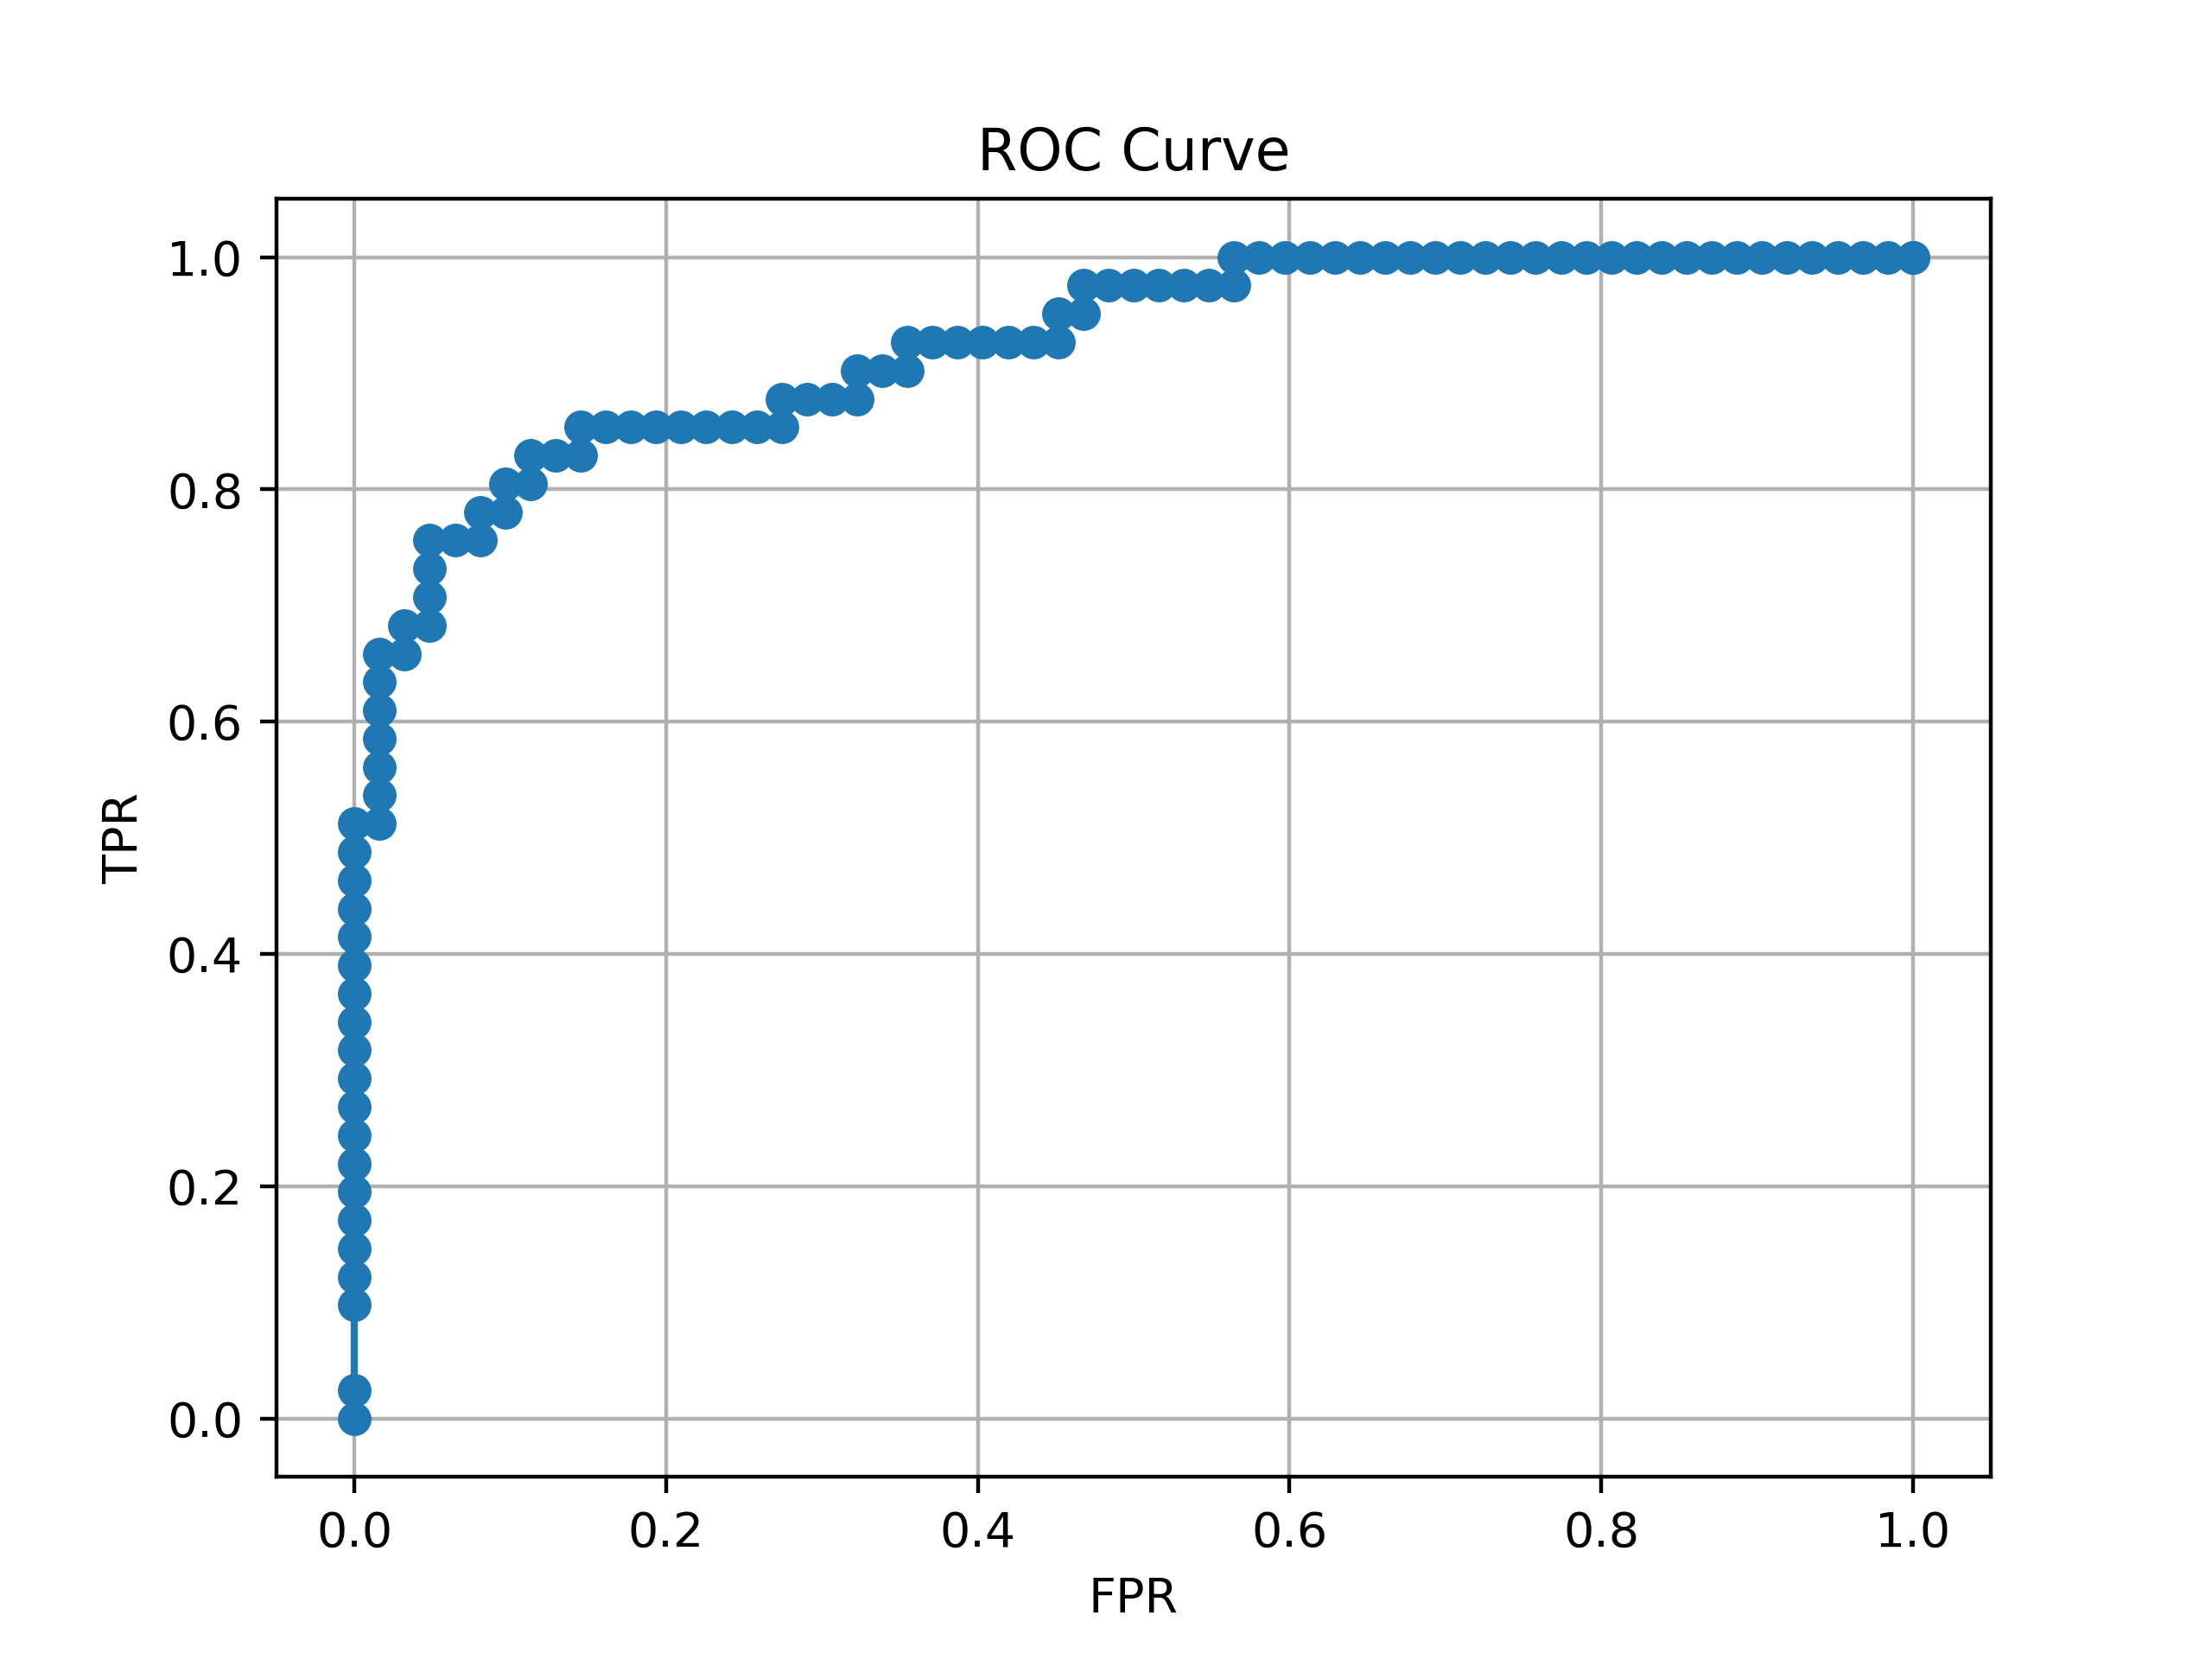
\includegraphics[width=0.6\textwidth]{src/roc_curve.png}
    \caption{ROC curve with feature selection}
    \label{fig:roc_fs}
\end{figure}

\begin{figure}[H]
    \centering
    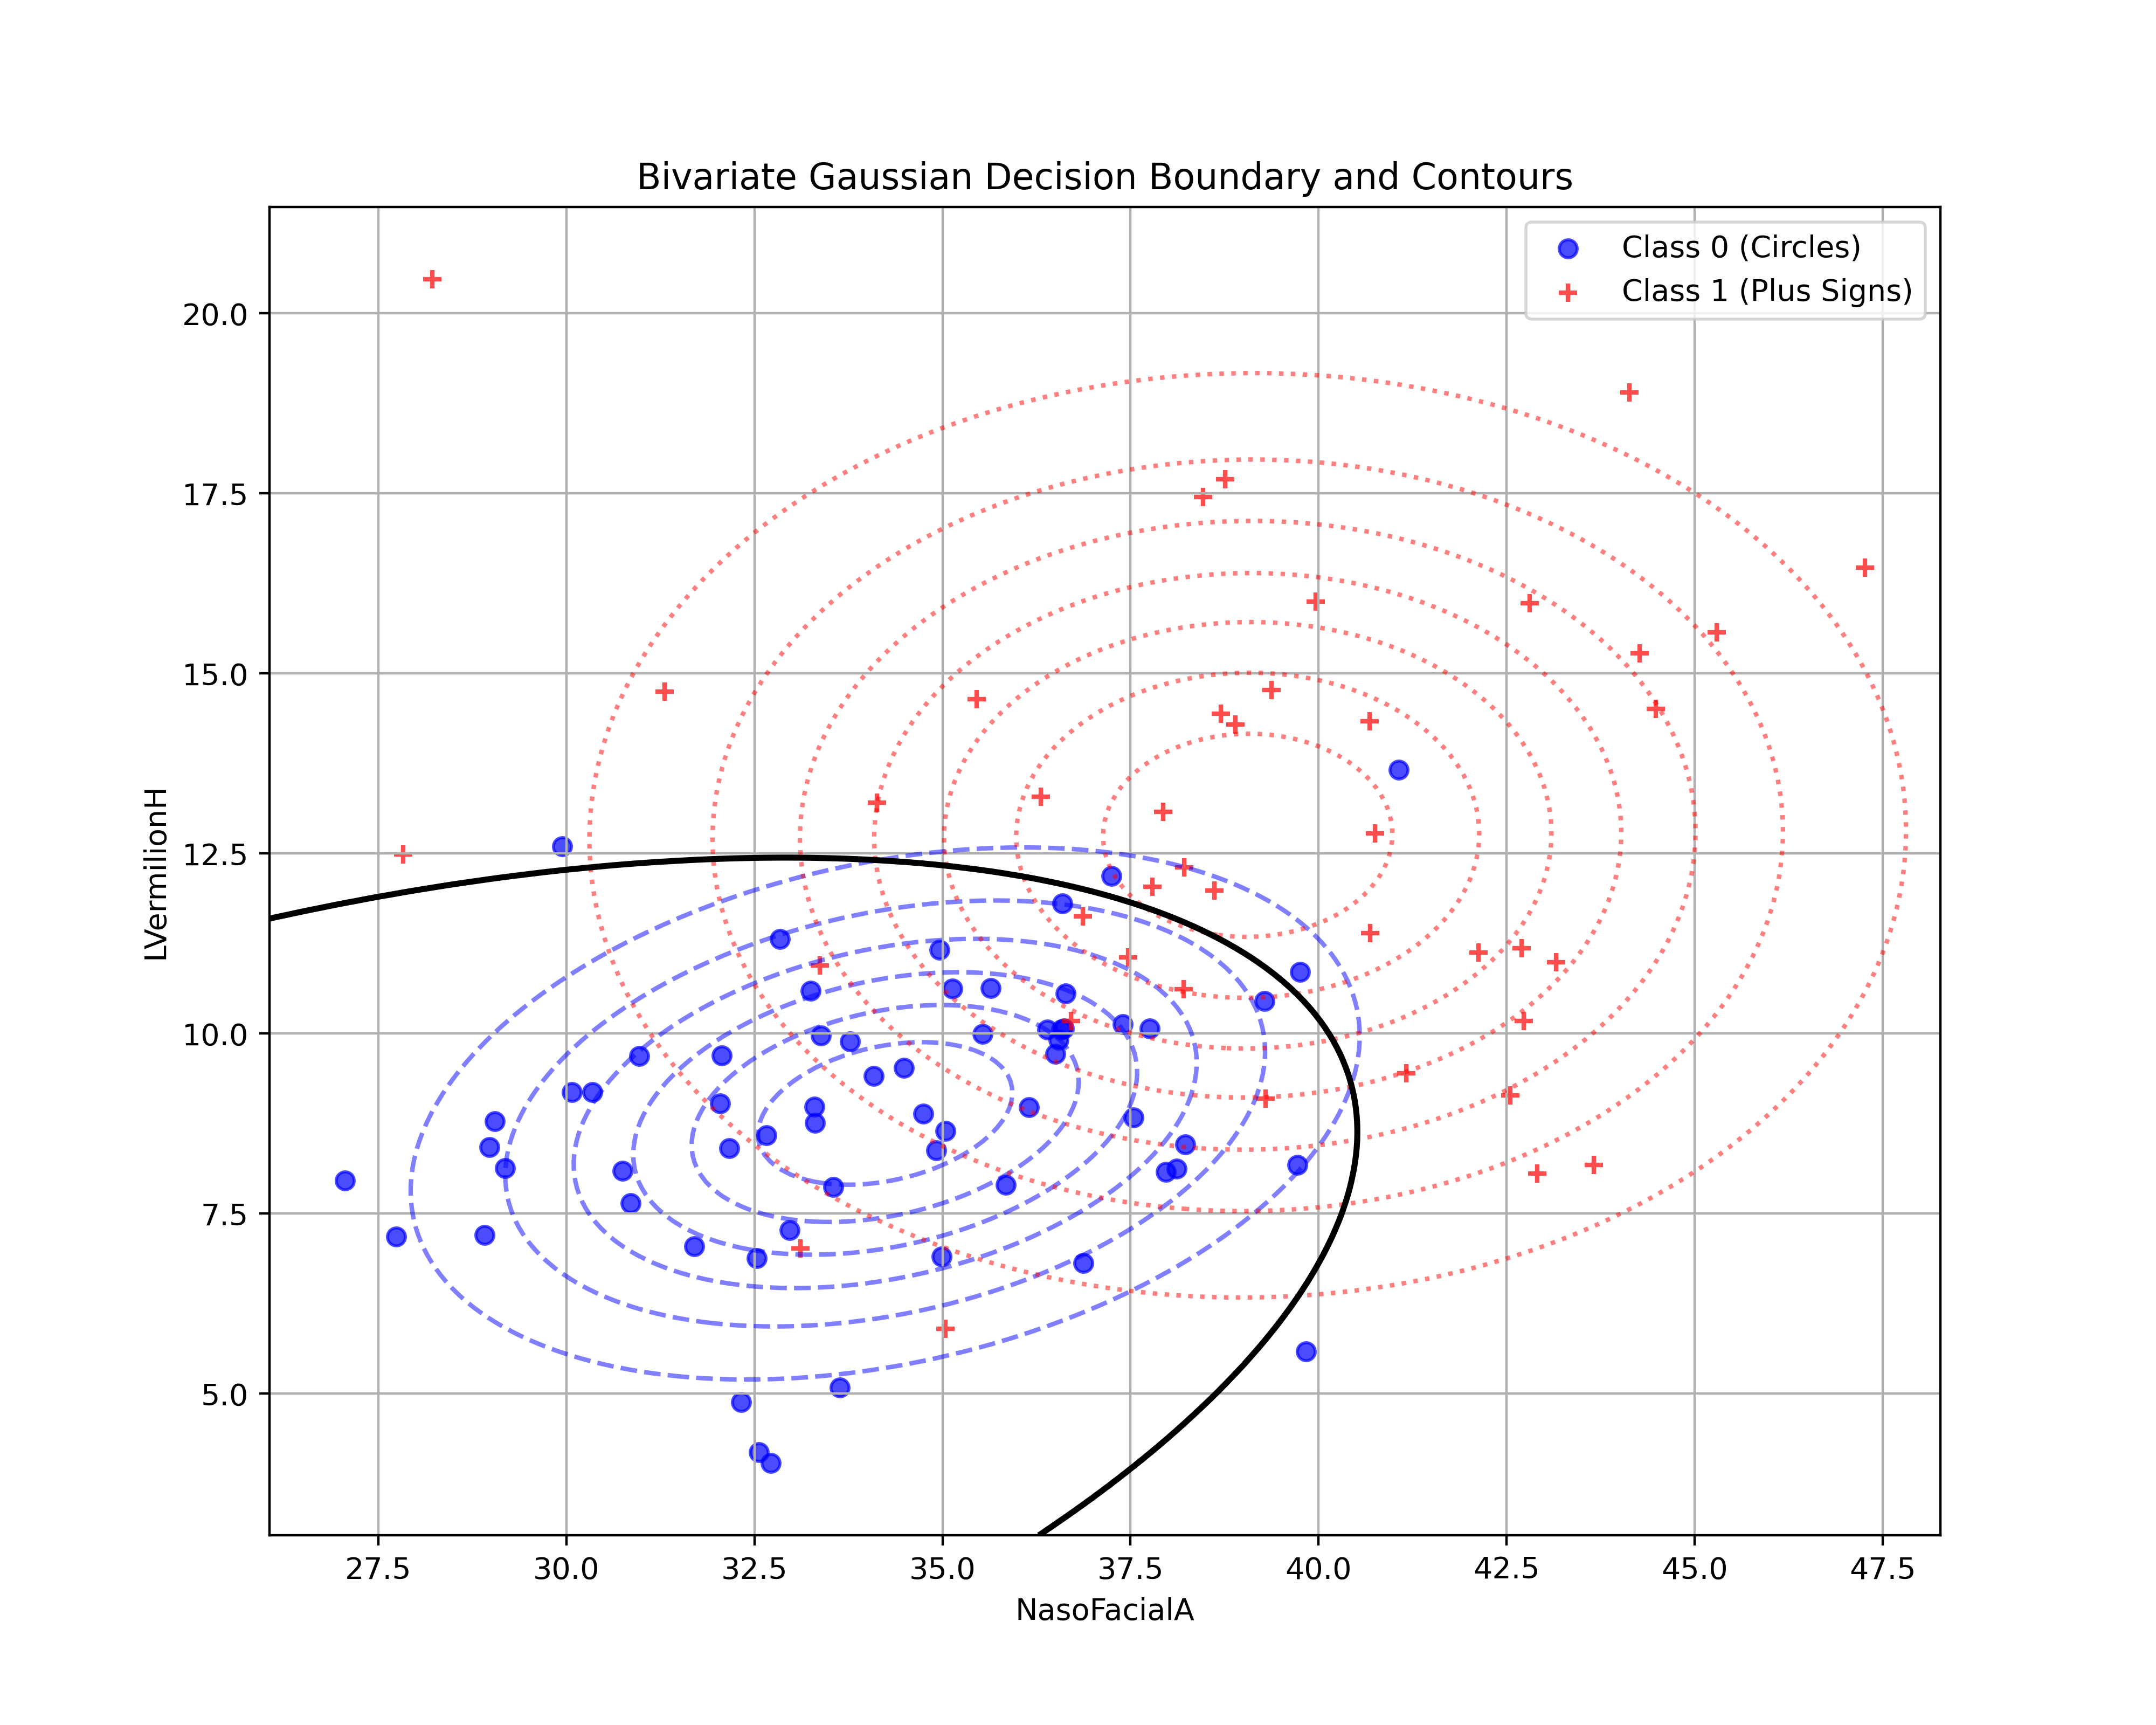
\includegraphics[width=0.6\textwidth]{src/decision_boundary_plot.png}
    \caption{Decision boundary with feature selection}
    \label{decision_boundary_fs}
\end{figure}

\subsubsection{Others}

\subsection{Random Forest Classifier}
\subsubsection{Model Description}
In this homework, I implement a Random Forest Classifier to classify data points based on their features. The model constructs a multitude of decision trees during training and outputs the mode of the classes (classification) of the individual trees.

\section{Problem 2}


\end{document}